\documentclass{article}
\usepackage{graphicx}
\graphicspath{{./Figures/}}
\usepackage{geometry}
\usepackage[pdfauthor={Farboud Khatami},
            pdftitle={Sydney Str User Manual},
            pdfsubject={User Manual},
            pdfkeywords={Structural Analysis},
            colorlinks=true]{hyperref}
            
\begin{document}
\centerline{\sc \large SYDNEY STR.}
\vspace{.5pc}
\centerline{\sc \large User Manual}
\centerline{\sc  \large (2013)  Farboud Khatami / Ehsan Torkaman}
\vspace{2pc}

Sydney Structure is a retro-styled 2-D frame analysis programme, using the matrix analysis method. The programme supports temperature effects, build errors and support deflections as well as the usual loadings. Sydney Str. also features a unique graphic part where the user can see the structure and its members’ deflections, check the input data, and even print the structure if necessary.

The programme is compiled using the Intel(c) visual Fortran compiler. Sydney Str. is made as a structural analysis II course project and is for educational purposes ONLY. 
       
\section{HOW TO USE SYDNEY STR. }
Since using this programme involves inputting a lot of data, some might find using it a bit challenging. Inputting a lot of data means a lot of potential user mistakes. So it is recommended for all users to read this manual before using the programme to avoid any probable misunderstanding of the commands.
	This guide contains a step-to-step explanation of what users confront during the use.
\section{SCREEN SETUP}
In this part you will be asked for the maximum structure dimensions (i.e the height and the length). These data will be used to adjust the graphic screen so that the structure can fit through. Note that the x-axis and y-axis scales will not necessarily be the same. If intended to use the same scales, the user should input the same number as the answer to both questions that are asked by the programme in this section (And this number is obviously the largest of both height and length).
Since the two mentioned scales may not be the same, the drawn gridlines may not form “squares”. Also, for large mumbers the gridlines are not drawn completely to help the user see the structure better.
\section{NODES}
The number of the nodes is asked. Knowing the number of nodes, the programme automatically asks for their x and y co-ordinates. The co-ordinate are relative to the graphics window’s lower left corner. You can input negative co-ordinates; but since the graphic window is adjusted to work with positive numbers, it is strongly recommended to use positive numbers.
	
	Should the user makes a mistake in inputting the data, they can correct the number of nodes and their co-ordinates at the end of this section.
	
	After checking the data, pressing Return causes the screen to clear and the programme to proceed to the next step.
\section{ELEMENTS}
After determining the number of the elements, the user should input the number of the two nodes on the beginning and the end of each element. The order of these to nodes is not important, but the user should keep in mind the input order and element number for further use. Also, the order of entering the elements is not important.
	
	Once the two nodes of an element are set, that element will be drawn in the graphics window so that the user can check the data.
	
	Just like the “nodes” part, the input data can be corrected if necessary. At the end, pressing return causes the programme to proceed.
\section{SECTION PROPERTIES}	
In the next three parts the user will be asked for the members’ Area, Moment of inertia and Modulus of elasticity respectively. Just make sure that you remember the number of each member to avoid setting the section properties to a wrong member.
	These three parts do not contain any graphical effects.
	The input data is verified and changed (if necessary) after the completion of the third part (i.e. Modulus of elasticity).
\section{SUPPORTS}
Setting the member properties, the user will be asked for the number of the supports and their type. A list of available supports is available to the user. To determine the support type, the user can simply type the number next to the support type in the list. The supports, their identification code, and their visualization can also be seen in table ~\ref{tbl1}. Note that:
\begin{table}
\centering
\caption{Support Types}
\label{tbl1}
\begin{tabular}{|c|l|c|}
\hline ID & Support Name & Depiction\\
\hline 2 & Pin & 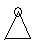
\includegraphics[height=.5cm]{pin.jpg}\\
\hline 3 & Roller (Horizontal) & 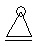
\includegraphics[height=.5cm]{rollerh.jpg}\\
\hline 3 & Roller (Vertical) &  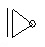
\includegraphics[height=.5cm]{rollerv.jpg}\\
\hline 3 &Roller (Tilted) & 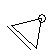
\includegraphics[height=.5cm]{rollert.jpg}\\
\hline 4 & Fixed & 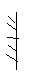
\includegraphics[height=.6cm]{fixed.jpg}\\
\hline 5 & Guided (Horizontal) & 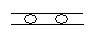
\includegraphics[height=.5cm]{guideh.jpg}\\
\hline 5 &Guided (Vertical) & 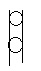
\includegraphics[height=.6cm]{guidev.jpg}\\
\hline 5 & Guided (Tilted) & 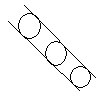
\includegraphics[height=.5cm]{guidet.jpg}\\
\hline
\end{tabular}
\end{table}
\begin{itemize}
\item The orientation of rollers and guided supports will be asked after their definition.
\item You can NOT allocate more than one support to a node.
\end{itemize}
Upon allocation, the supports are drawn in the window to the right. Just note that the visualization of the tilted supports may not be what you have in mind, but it doesn’t affect the programme calculations. Also, in some cases the supports are not displayed correctly (they might become stretched).

	The stability of the structure will be checked later automatically.
\section{LOADING}
Just like the previous part you can add loads to the structure by indicating the member number and load ID. Load IDs and a visualization is seen in table~\ref{tbl2}. The IDs can also be accessed via the programme.
\begin{table}
\centering
\caption{Load Cases}
\label{tbl2}
\begin{tabular}{|c|l|c|}
\hline ID & Load Case & Depiction\\
\hline 1 &Concentrated Perpendicular Load& 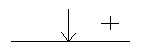
\includegraphics[height=.5cm]{cpl.jpg}\\
\hline 2 &Distributed Uniform Perpendicular Load & 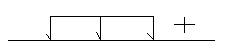
\includegraphics[height=.5cm]{dupl.jpg}\\
\hline 3 & Whole-span Triangular Load (Max to the left) &  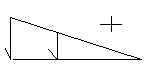
\includegraphics[height=.5cm]{wtll.jpg}\\
\hline 3 &Whole-span Triangular Load (Max to the right) & 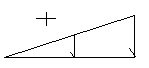
\includegraphics[height=.5cm]{wtlr.jpg}\\
\hline 4 &Concentrated Moment & 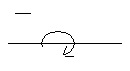
\includegraphics[height=.6cm]{cm.jpg}\\
\hline 5 & Concentrated Tangential Load & 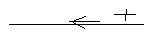
\includegraphics[height=.5cm]{ctl.jpg}\\
\hline 6 &Distributed Uniform Tangential Load & 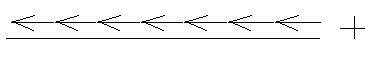
\includegraphics[height=.6cm]{dutl.jpg}\\
\hline
\end{tabular}
\end{table}
If the load you want to allocate is not in the list above, you can enter it using the principle of superposition. In this case you should add the minor loads (that form the load you want) to the number of loaded elements.
Should you want to add nodal forces (or moments), you can use one of the loads above and set the location in a way that they are applied to a node.
All the loads are set relative to the member they are applied to. Keep in mind the first and second node of the load before applying the load. If the first node of the element is to the right side of the second node, then the signs shown in table~\ref{tbl2} are valid. Look at figure~\ref{p1}.
\begin{figure}
\centering
 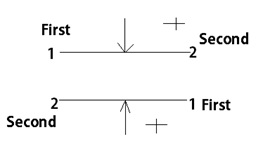
\includegraphics{loaddir.jpg}
 \caption{Load Directions}
 \label{p1}
 \end{figure}
 
 Since the loads are always relative to the members, for sidelong members you may need to break the load into two perpendicular axes.
 
 NOTE: The programme does NOT offer a visualization for the applied loads. So don’t go looking for them.
 \section{TEMPERATURE EFFECTS}
 The next step will be determining the probable temperature effects. The temperature effects can either be “Uniform” or “Gradient”. After setting the type, the additional required information will be asked for. Keep in mind that for the Gradient type, the top and the bottom of the element can be determined with respect to figure~\ref{p2}.
 \begin{figure}
\centering
 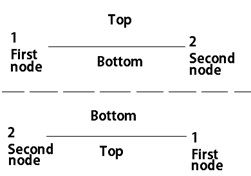
\includegraphics{bot.jpg}
 \caption{Member Bottom and Top}
 \label{p2}
 \end{figure}
 
 After the data verification, you can proceed to the next part.
 \section{SUPPORT DEFLECTIONS }
 The support deflections can ONLY be rotational or in the y-axis (in the global co-ordinate system). No more than one deflection can be allocated to a node. The positive deflection signs are just OPPOSITE the positive force signs.
  \begin{figure}
\centering
 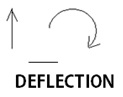
\includegraphics{ndef.jpg}
 \caption{Negative Deflections}
 \label{p3}
 \end{figure}
 \section{BUILD ERROR}
 The last step in inputting the data will be setting the build errors. Build errors occur when the actual length of an element differs from the designed length. In theory, build errors are not a far cry from uniform temperature effects. So handling this part is just like dealing with the uniform temperature change part.
 \section{OUTPUT}
 With all the required data provided for the programme, the calculation part is automatically done by the machine. After the calculation part a list of nodes and their corresponding forces (Fx, Fy, and Moment) appears. An identical copy of this list is also printed to a .txt file that can be found in the same folder as the programme. By pressing return, the screen clears and an another list appears. The second list is exactly the same as the first one, but shows the deflections. At this point, an approximate depiction of the displaced frame is also drawn in the window to the right. The mentioned drawing does NOT show the actual displaced frame; as the members are drawn as DIRECT LINES and the rotations are NOT illustrated correctly. The displacements are also included in the .txt file.
You can also save the contents of the graphic window as a .bmp file. Printing the contents of the graphic window is also possible. In order to do so, you need to select the graphic window by clicking on it and access the “Print” or “Save” options via the “File” tab. 
Note that you can print or save the contents of both windows anytime you wish (even before the output part).
After this part, pressing return shows the last window which terminates the programme.

Be sure to check the “Help” tab if you needed extra information about options available to you.
\section{CREDITS}
\subsection{Personel}
\begin{tabular}{ll}
Design\\
Graphics\\
Programming & Farboud Khatami\\
\\
Test\\
Programming\\
Matrix Analysis Help & Ehsan Torkaman\\
\end{tabular}

\subsection{Licence}
This program is	a product of Farboud Khatami and Ehsan Torkaman. It is distributed under AGPL V3 licence.

\section{DISCLAIMER}

The author and publisher of this program make no warranty of any
kind either expressed or implied. In particular we make no
warranty as to correctness or fitness for a particular purpose.

In no event shall the author or publisher be liable for any errors
contained herein or for incidental or consequential damages in
connection with the furnishing, performance, or use of this product
or documentation.

The information in this document is subject to change without
notice.


\end{document}